\documentclass[12pt]{exam}
\usepackage{amsthm}
\usepackage{libertine}
\usepackage[utf8]{inputenc}
\usepackage[margin=1in]{geometry}
\usepackage{amsmath,amssymb}
\usepackage{multicol}
\usepackage[shortlabels]{enumitem}
\usepackage{siunitx}
\usepackage{cancel}
\usepackage{caption}
\usepackage{graphicx}
\usepackage{pgfplots}
\usepackage{listings}
\usepackage{tikz}


\pgfplotsset{width=10cm,compat=1.9}
\usepgfplotslibrary{external}
\tikzexternalize

\newcommand{\class}{Laboratorio Física II} % This is the name of the course 
\newcommand{\examnum}{Laboratorio 13} % This is the name of the assignment
\newcommand{\examdate}{29/11/2022} % This is the due date
\newcommand{\timelimit}{}
\newenvironment{Figura}
  {\par\medskip\noindent\minipage{\linewidth}}
  {\endminipage\par\medskip}




\begin{document}
\pagestyle{plain}
\thispagestyle{empty}

\noindent
\begin{tabular*}{\textwidth}{l @{\extracolsep{\fill}} r @{\extracolsep{6pt}} l}
\textbf{\class} & \textbf{Name:} & \textit{David Pachon Ballen}\\ %Your name here instead, obviously 
\textbf{\examnum} &&\textit{Sergio Montoya Ramírez}\\
\textbf{\examdate} &&\\
\end{tabular*}\\
\rule[2ex]{\textwidth}{2pt}
% ---


\begin{multicols}{2}
\section{Objetivos}
\begin{itemize}
\item Estudiar el campo magnético producido por un solenoide
\item Medir la constante de permeabilidad magnética del vacío, $\mu_0$.
\item Usar el principio de superposición vectorial en campos magnéticos para obtener la magnitud de la dirección 
Norte del campo magnético terrestre.
\end{itemize}
\section{Introducción}
El movimiento de cargas eléctricas, ya sea por corrientes
(como en el alambre de una inductancia) o por movimiento 
de electrones en orbitales atómicos (como en un imán
permanente), genera fuerzas que se describen mediante
campos magnéticos. Como ejemplo, tenemos que el movimiento
 de aleaciones de hierro fundido al interior de la
tierra genera un campo magnético conocido como campo 
geomagnético. Recordemos que como campo vectorial,
este tiene una magnitud y dirección asociadas en cada
punto del espacio. La interacción entre este y un material 
imantado permitirá el funcionamiento de una brújula
cuya dirección se alinea a la del campo magnético terrestre.
 Un sensor de campo magnético nos permite medir la
magnitud del mismo en un punto en el espacio; en nuestro 
caso, haremos uso de un sensor de campo magnético
de tres ejes que nos permite reconstruir los vectores que
lo conforman. Con esto en mente, en la presente práctica
usaremos este sensor para: 
\begin{enumerate}
  \item medir la constante de 
  permeabilidad magnética del vacío,
  \item medir la componente
  Norte del campo magnético terrestre.
\end{enumerate}
\section{Analisis Cualitativo}
\begin{enumerate}
\item Si se desea construir un dispositivo que cancele
 el campo magnético externo usando solenoides,
¿cuántos solenoides son necesarios para cancelar el
campo magnético externo? ¿Qué aplicaciones tiene el
poder cancelar el campo magnético externo?

\textbf{Solución: }Dadas las caracterizticas de los solenoides asumiendo uno perfecto
entonces no deberiamos necesitar otro para cancelarlo pues este ya
intenta evitar que el campo afuera sea grande.

\item ¿Cómo es el comportamiento de la brújula al aumentar la corriente en el alambre? Explique.

\textbf{Solución: } Al aumentar la corriente se genera un campo magentico mas potente que causa que la brujula
cambie de posición y dirección a la que apunta.

\item En el procedimiento experimental se pide ubicar la
brújula en el centro del aro, ¿por qué es esto conveniente?

\textbf{Solución: } Esto es dado que de esa manera los efectos del campo magnetico son simetricos y por tanto
sus efectos son mas claros.

\item  ¿Qué efecto tendría aumentar el número de vueltas
del aro? ¿Cómo cambiaría la gráfica Ba vs. I?

\textbf{Solución: } Como el numero de vueltas es directamente proporcional al campo entonces sus efectos serian mas grandes.
En concreto, nos referimos a la ecuación (7) que es $B_a = N\frac{\mu I}{2 R}$

\item ¿Qué efecto tendría intercambiar los cables conectados a la fuente en el campo magnético producido por
el aro?

\textbf{Solución: } Pues esto haria que la corriente tuviera un sentido opuesto y por tanto por ley de la mano derecha
los efectos del mismo serian opuestos en dirección.

\item ¿Qué efecto tendría en el experimento que el campo
del aro no se genere de forma perpendicular al campo
magnético terrestre?

\textbf{Solución: } Como el campo es un vector en ambos casos entonces lo que ocurriria es que estos interferirian
constructivamente y por tanto el efecto se amplificaria.
\end{enumerate}
\section{Analisis Cuantitativo}
\begin{Figura}
    \centering
    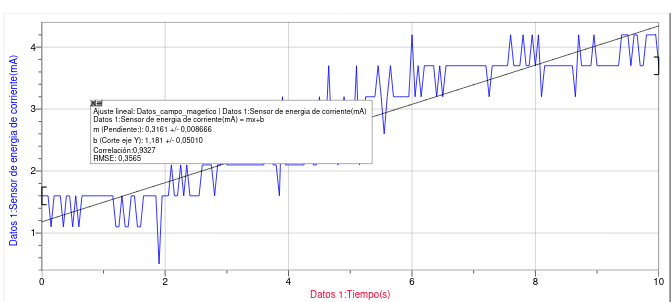
\includegraphics[width=0.9\textwidth]{Figura_1_Lab13.png}
    \captionof{figure}{Datos de corriente vs Tiempo en el primer solenoide}
    \label{fig}
\end{Figura}
\begin{Figura}
  \centering
  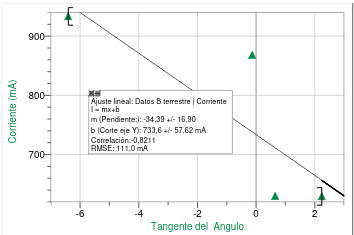
\includegraphics[width=0.9\textwidth]{Figura_2_Lab13.png}
\end{Figura}
\section{Conclusión}
El objetivo del laboratorio fue el de medir la constante de permeabilidad magnética del vacío,
 $\mu_0$. Y obtener la magnitud de la dirección norte del campo magnético terrestre. Lo primero
  lo logramos con un buen número de datos de bace y con la formula 13.1. Obteniendo el campo 
  magnético de la regresión lineal sobre la gráfica de corriente vs tiempo. 
  Este último fue de $0,3161 +/- 0,008666$ mT. El valor que obtuvimos para la constate de permeabilidad 
  magnética del vacío fue de $0.000087 +/- 1x10**(-5) NA^{-2}$. Siendo el valor teórico de la última $0,000001257 NA^{-2}$ 
  tenemos un error relativo porcentual de $6821.241\%$ o mejor entenderlo como un orden de magnitud por encima de lo esperado.
Para la magnitud de la dirección norte del campo magnético terrestre hicimos una gráfica de corriente vs tangente del ángulo. 
Sobre la mencionada gráfica, hicimos una regresión cuya pendiente es el valor en magnitud el buscado y dio $34,39 +/- 16,90 \mu T$ siendo el teórico 
27,0 µT. Lo último nos da un error relativo porcentual de $27.37 \%$.
$$B_{sol} = N \frac{\mu_0 I}{L}$$
\end{multicols}2

\end{document}
